\documentclass[../main.tex]{subfiles}
\graphicspath{{\subfix{../images/}}}
\begin{document}

\subsection*{Answers - Volumes of revolution (page \pageref{Volumes of revolution})}
\label{Volumes of revolution answers}
\begin{spacing}{1.5}

\begin{enumerate}[itemsep=0.7cm]
    \item 
    $V=\pi \int_0^{\frac{\pi}{2}} \cos^2{x}\,dx$

    Using $\cos{2x}=2\cos^2{x}-1$:

    $V=\pi \int_0^{\frac{\pi}{2}} \Bigl(\frac{\cos{2x}}{2}+\frac{1}{2}\Bigr)\, dx$

    $V=\Bigl[\frac{\sin{2x}}{4}+\frac{x}{2}\Bigr]_0^{\frac{\pi}{2}}$

    $V=\frac{\pi^2}{4}=2.467$

    \item 
    $V=\pi \int_0^4 (x^{\frac{1}{3}})^2\,dx$

    $V=\pi \int_0^4 x^{\frac{2}{3}}\, dx$

    $V=\pi \Bigl[\frac{3}{5}x^{\frac{5}{3}} \Bigr]_0^4$

    $V=6.05\pi = 19$

    \item
    $V=\pi \int_0^4 (20-x^2)^2\, dx$

    $V=\pi \int_0^4 (400-40x^2+x^4)\,dx$

    $V=\pi \Bigl[400x-\frac{40}{3}x^3+\frac{x^5}{5} \Bigr]_0^4$

    $V=\frac{14272}{15}\pi=2989$

    \item 
    Since it is rotated around the y-axis, we need to rearrange the function:

    $\frac{4}{3}y=\sqrt{16-x^2}$

    $\frac{16}{9}=16-x^2$

    $x^2=16-\frac{16}{9}$

    Now we can insert this into the volume of revolution formula:

    $V=\pi \int_0^3 (16-\frac{16}{9})\,dy$

    $V=\pi \Bigl[16y-\frac{16}{27}y^3\Bigr]_0^3$

    $V=32\pi$

    \item 
    
    \begin{enumerate}
        \item 
        $V=\pi \int_0^8 (x+a)\,dx$

        $V=\pi \Bigl[\frac{x^2}{2}+ax\Bigr]_0^8$

        $V=\pi[32+8a]=32\pi+8a\pi$

        \item 
        $32\pi + 8a\pi=200$

        $8a\pi=200-32\pi$

        $a=\frac{200-32\pi}{8\pi}=3.96$

    \end{enumerate}
    
    \item 
    Since we are rotating around a vertical axis, we need to rearrange to make $x$ the subject:

    $x=e^y$

    Then we shift the curves and axis of rotation $\frac{1}{e}$ to the left so that the axis of rotation returns to the $y$-axis.

    $x=e^y-\frac{1}{e}$

    $V=\pi \int_{-1}^1 \Bigl(e^y -\frac{1}{e}\Bigr)^2\,dy$

    $V=\pi \int_{-1}^1 \Bigl(e^{2y}-2e^{y-1}+\frac{1}{e^2}\Bigr)\,dy$

    $V=\pi \Bigl[\frac{e^{2y}}{2}-2e^{y-1}+\frac{y}{e^2}\Bigr]_{-1}^1$

    $V=\pi \Bigl[\Bigl(\frac{e^2}{2}-2+\frac{1}{e^2}\Bigr)-\Bigl(\frac{1}{2e^2}-\frac{2}{e^2}-\frac{1}{e^2}\Bigr)\Bigr]$

    $V=6.812$

    \item 
    It is a vertical axis, so we need to make $x$ the subject:

    $x=e^y$

    Then we shift the axis 1 to the right, back to the $y$-axis.

    $x=e^y+1$

    $V=\pi \int_0^2 (e^y +1)^2\,dy$

    $V=\pi \int_0^2 (e^{2y}+2e^y+1)\,dy$

    $V=\pi \Bigl[\frac{e^{2y}}{2}+2e^y+y\Bigr]_0^2$

    $V=\pi \Bigl[(\frac{e^4}{2}+2e^2+2)-(\frac{1}{2}+2+0)\Bigr]$

    $v=130.6$

    \item 
    Translate both functions up by 1 so that the axis of rotation is back at the $x$-axis:

    $y=\sqrt{x}+1$

    $y=x+1$

    Find the boundaries:

    $\sqrt{x}=x\\
    x=x^2\\
    x^2-x=0\\
    x(x-1)=0$

    Boundaries are at $x=0, 1$

    $V=\pi \int_0^1 (\sqrt{x}+1)^2-(x+1)^2\,dx$

    $V=\pi \int_0^1 \Bigl(x+2\sqrt{x}+1-x^2-2x-1\Bigr)\,dx$

    $V=\pi \int_0^1 \Bigl(-x^2 -x+2\sqrt{x}\Bigr)\,dx$

    $V=\pi \Bigl[-\frac{x^3}{3}-\frac{x^2}{2}+\frac{4}{3}x^{\frac{3}{2}}\Bigr]_0^1$

    $V=\pi \Bigl[(-\frac{1}{3}-\frac{1}{2}+\frac{4}{3}-(0))\Bigr]=\frac{\pi}{2}$

    \item 
    $V=\pi \int_0^h 4ax\,dx$

    $V=\pi \Bigl[2ax^2\Bigr]_0^h$

    $V=\pi [2ah^2 - 0]$

    $V=2ah^2\pi$

    \item 
    \begin{enumerate}
        \item 
        $V=\pi \int_0^{\ln{(p)}} \phi(e^{-x}-e^{-2x})\,dx$
    
        $V=\pi \phi\int_0^{\ln{(p)}} (e^{-x}-e^{-2x})\,dx$
    
        $V=\pi \phi \Bigl[-e^{-x}+\frac{e^{-2x}}{2}\Bigr]_0^{\ln{(p)}}$

        $V=\pi \phi \Bigl[\Bigl(-e^{-\ln{(p)}}+\frac{e^{-2\ln{(p)}}}{2}\Bigr)-\Bigl(-1+\frac{1}{2}\Bigr)\Bigr]$

        $V=\pi \phi \Bigl(-\frac{1}{p}+\frac{1}{p^2}+\frac{1}{2}\Bigr)$

        $V=\frac{\pi \phi}{2}\Bigl(-\frac{2}{p}+\frac{1}{p^2}+1\Bigr)$

        $V=\frac{\pi \phi}{2}\Bigl(\frac{-2p+1+p^2}{p^2}\Bigr)$

        $V=\frac{\pi \phi}{2}\Bigl(\frac{p-1}{p}\Bigr)^2$
    
        \item Since $p-1<p$ we know that $\frac{p-1}{p}$ is between zero and 1. That means that $\Bigl(\frac{p-1}{p}\Bigr)^2$ will always be less than one, so no matter how large $p$ gets, $V<\frac{\pi \phi}{2}$
    
    \end{enumerate}
    
    \item 
    A sketch of the shape in 2D, (rotated 90$^\circ$ to make it easier to visualise):

    \begin{figure}[h!]
        \centering
        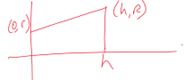
\includegraphics{images/volrev20.png}
    \end{figure}

    $y=mx+c$

    $m=\frac{R-r}{h}$

    $y=\Bigl(\frac{R-r}{h}\Bigr)x+r$

    $V=\pi \int_0^h \Bigl[\Bigl(\frac{R-r}{h}\Bigr)x+r\Bigr]^2\,dx$

    $V=\pi \int_0^h \Bigl((\frac{R-r}{h})^2x^2 +2(\frac{R-r}{h})rx+r^2\Bigr)\, dx$

    $V=\pi \Bigl[(\frac{R-r}{h})^2 \frac{x^3}{3}+(\frac{R-r}{h})rx^2+r^2x\Bigr]_0^h$

    $V=\pi \Bigl[\frac{R^2-2Rr+r^2}{h^2}\times \frac{h^3}{3}+\frac{Rr-r^2}{h}\times h^2 +r^2h\Bigr]$

    $V=\pi h\Bigl[\frac{R^2-2Rr+r^2}{3}+Rr-r^2+r^2\Bigr]$

    $V=\pi h\Bigl[\frac{R^2-2Rr+r^2}{3}+Rr\Bigr]$

    $V=\frac{\pi h}{3}\Bigl[R^2-2Rr+r^2+3Rr\Bigr]$

    $V=\frac{\pi h}{3}\Bigl[R^2+Rr+r^2\Bigr]$ (as required)

\end{enumerate}


\pagebreak
\end{spacing}

\end{document}